\section{GPU-Accelerated PNG Encoding}
\label{sec:gpu-png-encoding}

An expensive fractal calculation can finish before its image is ready to save: coloring,
compression, and file output are separate tasks. PNG encoding is therefore a useful secondary
application of GPU parallelism. FractalShark moves both coloring and lossless encoding onto the
GPU, then returns a complete PNG byte stream to the host. The mathematical image is unchanged;
the implementation changes how the same pixel data are packaged for storage.

\subsection{From a Rendered Frame to a PNG}
\label{subsec:png-output}

The save queue captures the iteration data, dimensions, and palette state needed by each request.
Both CPU and GPU saves run asynchronously; callers that require completed files must drain the
save queue. A GPU job leases a dedicated \code{GpuSaveEncoder} context and uses its own
nonblocking CUDA stream, so encoding work has separate buffers and ordering from interactive
rendering. The context retains workspace for subsequent images instead of allocating every
intermediate buffer anew.

\begin{figure}[htbp]
\centering
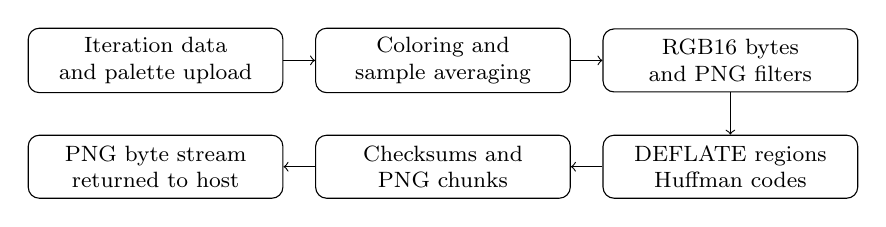
\begin{tikzpicture}[every node/.style={font=\footnotesize,align=center},
    box/.style={draw,rounded corners,minimum height=0.8cm,text width=3.0cm}]
\node[box] (capture) at (0,0) {Iteration data\\and palette upload};
\node[box] (color) at (3.65,0) {Coloring and\\sample averaging};
\node[box] (filter) at (7.3,0) {RGB16 bytes\\and PNG filters};
\node[box] (compress) at (7.3,-1.35) {DEFLATE regions\\Huffman codes};
\node[box] (frame) at (3.65,-1.35) {Checksums and\\PNG chunks};
\node[box] (return) at (0,-1.35) {PNG byte stream\\returned to host};
\draw[->] (capture) -- (color);
\draw[->] (color) -- (filter);
\draw[->] (filter) -- (compress);
\draw[->] (compress) -- (frame);
\draw[->] (frame) -- (return);
\end{tikzpicture}
\caption[GPU PNG encoding pipeline]{GPU PNG encoding pipeline. Disk output follows the
return of the completed byte stream and is a separate part of save latency.}
\label{fig:png-encoder-pipeline}
\end{figure}

Coloring converts iteration counts into red, green, and blue channels. Antialiasing averages
the colors of the samples belonging to one output pixel. PNG stores each 16-bit channel with
its most significant byte first, so one RGB16 pixel occupies six bytes
\cite{PNGThirdEdition2025}. Each scanline then
receives a filter tag followed by reversibly transformed bytes. These filters make neighboring
pixels easier to compress; they do not reduce channel precision.

For example, take two adjacent RGB16 pixels $(16,32,48)$ and $(17,33,49)$.
Their hexadecimal bytes are
\[
\underbrace{00\;10\;00\;20\;00\;30}_{\text{first pixel}}
\qquad
\underbrace{00\;11\;00\;21\;00\;31}_{\text{second pixel}}.
\]
The Sub filter replaces each byte by its difference, modulo 256, from the byte six positions
earlier. Missing bytes to the left are zero. The first pixel therefore remains unchanged,
whereas the second becomes $00\;01\;00\;01\;00\;01$. A decoder adds the previous pixel's
bytes back, modulo 256, recovering both pixels exactly. The same principle extends across
the scanline; other PNG filters exploit the preceding scanline as well.

\subsection{Parallel Lossless Compression}

After filtering, independent regions of at most 32\,KiB provide bounded work units for the
compressor. DEFLATE represents data with literal bytes and references to previously seen byte
sequences; Huffman codes give frequent symbols shorter bit representations \cite{RFC1951}.
The GPU can search
and encode many regions concurrently, then assemble their output in order. Region boundaries
limit the available matching history, so faster encoding can produce a larger file than a CPU
compressor with different search and block choices.

The encoder also computes the checksums required by the compressed stream and PNG chunks
\cite{RFC1950,PNGThirdEdition2025}.
Framing adds the PNG signature, image description, compressed image chunks, and end marker.
A valid decode must reproduce the intended channel values exactly, although two encoders can
emit different compressed bytes for those values. Pixel comparison after decoding, rather
than byte-for-byte comparison of the files, is the relevant correctness check. Reproduction
and validation commands are recorded in \cref{subsec:png-validation}.

\subsection{A Measured Speed--Size Tradeoff}
\label{subsec:png-benchmarks}

\begin{table}[htbp]
\centering
\begin{tabular}{lrr}
\hline
4K Mandelbrot fixture & GPU encoder & CPU encoder \\
\hline
Median encoding time & 13.12\,ms & 598.19\,ms \\
Completed PNG size & 857,686 bytes & 692,127 bytes \\
Reusable GPU workspace & approximately 265\,MiB & --- \\
\hline
\end{tabular}
\caption[Historical 4K PNG measurement]{Historical 4K PNG measurement from October 4, 2026,
for a $3840\times2160$ fixture in Windows Release on an RTX 5090 with CUDA runtime 13.2.
Three warm repetitions were summarized by their median.}
\label{tab:gpu-png-benchmarks}
\label{tab:png-current-benchmark}
\label{tab:png-compression-sizes}
\end{table}

The reported GPU encoding interval includes transfer of the completed compressed bytes to the
host. The comparison excludes input-color upload, CPU \code{WPngImage} construction, and disk
output; neither timing includes iteration upload or coloring. The retained workspace excludes
input and host buffers and the \code{GpuSaveEncoder} bridge buffers. The measurement therefore
covers encoding rather than the user's complete save operation. In this case the GPU encoder
was approximately 46 times faster and produced a file approximately 24 percent larger.
The result illustrates a useful tradeoff rather than a universal speedup: image content,
dimensions, hardware, and compression choices all affect the outcome. The retained workspace
also trades GPU memory for lower overhead on later saves.
